\documentclass[12pt]{article}



\usepackage{amsmath,amssymb,amsfonts}
\usepackage{graphicx}
\usepackage{geometry}
\usepackage{setspace}
\usepackage{booktabs}
\usepackage[numbers]{natbib}
\usepackage{caption}
\usepackage{subcaption}



\geometry{margin=1in}
\onehalfspacing



\title{Bayesian Estimation for the GIKw--Rayleigh Distribution\\
under Various Loss Functions}



\author{Dr. Nahid Sanjari\thanks{Corresponding author: \texttt{nsanjari@alzahra.ac.ir}} \\ Fatemeh Sanatian}



\date{February 21, 2026}



\begin{document}



\maketitle



\begin{abstract}
This document provides a comprehensive and self-contained treatment of Bayesian
estimation for the four-parameter Generalized Inverse Kumaraswamy–Rayleigh (GIKw–RD)
distribution. Starting from the probability density function, we derive the likelihood,
choose independent Gamma priors, and obtain the posterior distribution. Because
the posterior lacks a closed form, we present two widely used computational approaches:
Lindley's approximation and Markov Chain Monte Carlo (MCMC) with Metropolis-Hastings
steps. Detailed formulas are given for the Bayes estimators under Squared Error Loss
(SEL), Absolute Error Loss (AEL), LINEX Loss, and General Entropy Loss (GELF).
All necessary derivatives, expansions, and algorithmic steps are explicitly written out.
A simulation study illustrates the performance of the methods on two generated datasets.
\end{abstract}



\noindent\textbf{Keywords:} Bayesian estimation, GIKw-Rayleigh distribution,
Lindley approximation, MCMC, Loss functions, SEL, AEL, LINEX, GELF.



\section{Introduction}



The \textbf{Generalized Inverse Kumaraswamy–Rayleigh (GIKw–RD)} distribution is a
flexible lifetime model introduced in the literature to accommodate various shapes
of hazard rates and skewed data. Statistical distributions are prevalent in many
areas such as physics, computer science, insurance, communication etc. Due to the
random nature of the data arising in different fields, the well-established
distributions fail to provide an acceptable fit. Hence, several new generalizations
of existing models have been proposed. For example "Marshall-Olkin-G family" by
Marshall and Olkin (1997), "Kumaraswamy family-G" by Cordeiro and de Castro (2011),
"The gamma generated family" by Zografos and Balakrishnan (2009), "A new method of
Generating Families of distributions" by Alzaatreh et al. (2013), "Kumaraswamy
Transmuted-G family of distribution" by Afify et al. (2016a), "Kumaraswamy odd log
logistic Distribution" by Alizadeh et al. (2015a), "Weibull-G" by Bourguignon et al.
(2014), "Kumaraswamy Marshall-Olkin" by Alizadeh et al. (2015b), "Generalized
Transmute-G family" by Nofal et al. (2017), "Burr X-G" by Yousof et al. (2016),
"The Transmuted Geometric-G family" by Afify et al. (2016b), "Type I Half logistic
family" by Cordeiro et al. (2016) etc.



The inverted Kumaraswamy Distribution (IKwD) was introduced by Al-Fattah et al. (2017).
He expounded some of the properties of IKwD. Recently, Jamal et al. (2019) proposed
"Generalized Inverted Kumaraswamy Generated Family of Distribution" (GIKw-G). The
cdf and pdf of a GIKw-G family are given by (1) and (2) respectively.



\[
M(x) = \left\{1 - \left(1 - F^{\gamma}(x)\right)^{\alpha}\right\}^{\beta}; \quad \alpha,\beta,\gamma > 0
\]



\[
m(x) = \alpha\beta\gamma f(x)F^{\gamma-1}(x)(1 - F^{\gamma}(x))^{\alpha-1}
\{1 - (1 - F^{\gamma}(x))^{\alpha}\}^{\beta-1} \qquad (1)
\]



where \(F(x)\) and \(f(x)\) are the cdf and pdf of baseline distribution respectively.



The Rayleigh Distribution was introduced by Rayleigh (1880). Siddiqui (1962) studied
properties of Rayleigh distribution. Some other authors who also studied this model
are Merovci (2013), Ahmad et al. (2014), Howlader and Hossain (1995), Malik and Ahmad
(2019) etc.



The main aim of this paper is to generalize RD using GIKw-G family so that the
flexibility of RD can be enhanced in terms of density function and hazard rate.
The new distribution is named GIKw-Rayleigh Distribution (GIKw-RD) following the
approach of Malik and Ahmad (2024). The new distribution exhibits more complex
shapes of hazard rate function (hrf) and also outperforms some well-known
distributions in terms of two real life data sets. The rest of the paper is
organized as follows: In Section 2, the pdf, cdf and the associated reliability
measures of the new model are obtained. Section 3 and 4 deal with the structural
properties and stress strength reliability of the proposed model are derived.
The L-moments and estimation of parameters are discussed in section 5 and 6
respectively. Finally in section 7, the applicability of the model is established
by using two real life data sets.



\section{The GIKw–Rayleigh Distribution}



\subsection{Probability Density Function}



For a single observation \(x > 0\), the PDF is



\[
\begin{aligned}
f(x|\alpha,\beta,\gamma,\theta)
&= \alpha\beta\gamma \frac{x}{\theta^2}
\exp\left(-\frac{x^2}{2\theta^2}\right)
\left(1-e^{-\frac{x^2}{2\theta^2}}\right)^{\gamma-1} \\
&\quad\times \left(1-\left(1-e^{-\frac{x^2}{2\theta^2}}\right)^{\gamma}\right)^{\alpha-1}
\left[1-\left(1-\left(1-e^{-\frac{x^2}{2\theta^2}}\right)^{\gamma}\right)^{\alpha}\right]^{\beta-1},
\end{aligned}
\]



with \(\alpha,\beta,\gamma,\theta > 0\).



To simplify notation we introduce three auxiliary functions:



\[
A(\theta,x) = 1-e^{-\frac{x^2}{2\theta^2}},\qquad
B(\alpha,\gamma,\theta,x) = 1 - A(\theta,x)^{\gamma},\qquad
C(\alpha,\beta,\gamma,\theta,x) = 1 - B(\alpha,\gamma,\theta,x)^{\alpha}.
\]



For a sample \(\mathbf{x} = (x_1,\dots,x_n)\) we denote



\[
A_i = A(\theta,x_i),\quad B_i = B(\alpha,\gamma,\theta,x_i),\quad C_i = C(\alpha,\beta,\gamma,\theta,x_i).
\]



Then the PDF can be written compactly as



\[
f(x_i|\zeta) = \alpha\beta\gamma \frac{x_i}{\theta^2}
e^{-\frac{x_i^2}{2\theta^2}} A_i^{\gamma-1} B_i^{\alpha-1} C_i^{\beta-1},
\qquad \zeta = (\alpha,\beta,\gamma,\theta).
\]



\subsection{Likelihood Function}



Assuming independent observations, the likelihood is



\[
L(\zeta|\mathbf{x}) = \prod_{i=1}^{n} f(x_i|\zeta).
\]



Substituting the expression:



\[
L(\zeta|\mathbf{x}) = (\alpha\beta\gamma)^n \theta^{-2n}
\exp\left(-\frac{1}{2\theta^2}\sum_{i=1}^{n}x_i^2\right)
\times \prod_{i=1}^{n} A_i^{\gamma-1} B_i^{\alpha-1} C_i^{\beta-1}.
\]



The log-likelihood \(\ell(\zeta) = \ln L(\zeta|\mathbf{x})\) is



\[
\begin{aligned}
\ell(\zeta) = &\ n(\ln\alpha+\ln\beta+\ln\gamma) - 2n\ln\theta
- \frac{1}{2\theta^2}\sum_{i=1}^{n}x_i^2 \\
&+ (\gamma-1)\sum_{i=1}^{n}\ln A_i
+ (\alpha-1)\sum_{i=1}^{n}\ln B_i
+ (\beta-1)\sum_{i=1}^{n}\ln C_i.
\end{aligned}
\label{eq:loglik}
\]



\begin{figure}[htbp]
\centering
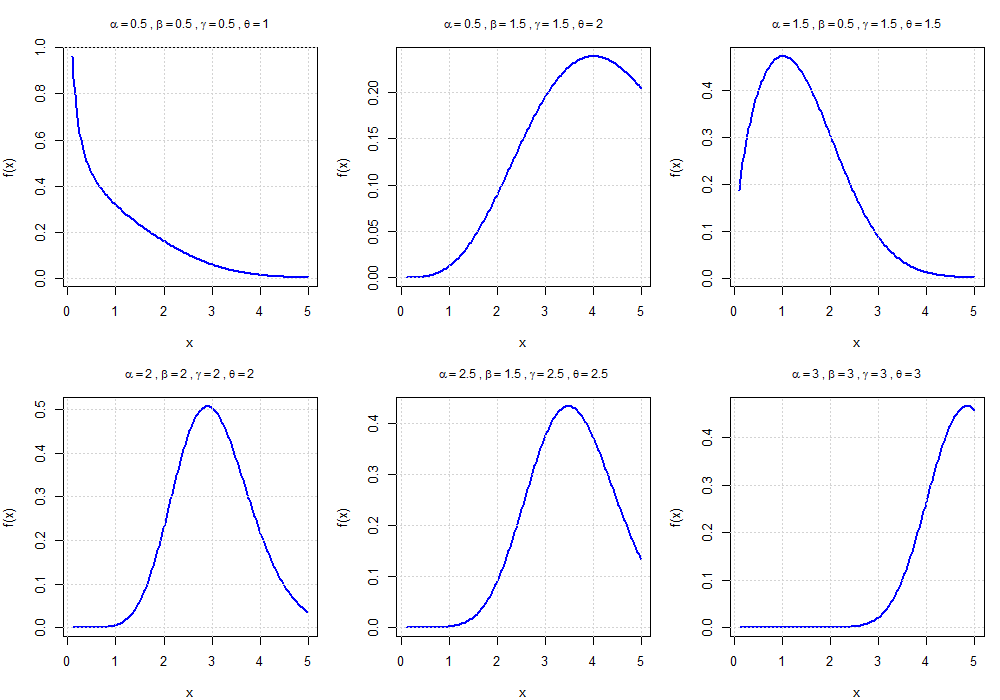
\includegraphics[width=0.8\textwidth]{Figure_1_PDF_GIKw_RD.png}
\caption{Probability Density Function of GIKw-RD for different parameter combinations.}
\label{fig:pdf}
\end{figure}



\section{Prior Distributions}



For the four positive parameters we choose independent Gamma priors as is common
in Bayesian analysis (Gelman et al., 2013):



\[
\begin{aligned}
\alpha &\sim \text{Gamma}(a_1,b_1), \quad
\pi(\alpha) \propto \alpha^{a_1-1}e^{-b_1\alpha},\\
\beta &\sim \text{Gamma}(a_2,b_2), \quad
\pi(\beta) \propto \beta^{a_2-1}e^{-b_2\beta},\\
\gamma &\sim \text{Gamma}(a_3,b_3), \quad
\pi(\gamma) \propto \gamma^{a_3-1}e^{-b_3\gamma},\\
\theta &\sim \text{Gamma}(a_4,b_4), \quad
\pi(\theta) \propto \theta^{a_4-1}e^{-b_4\theta},
\end{aligned}
\]



where \(a_i,b_i>0\) are hyperparameters. The joint prior is the product:



\[
\pi(\zeta) \propto \alpha^{a_1-1}\beta^{a_2-1}\gamma^{a_3-1}\theta^{a_4-1}
e^{-(b_1\alpha+b_2\beta+b_3\gamma+b_4\theta)}.
\]



\section{Posterior Distribution}



By Bayes' theorem, the joint posterior is proportional to likelihood times prior:



\[
\pi(\zeta|\mathbf{x}) \propto L(\zeta|\mathbf{x})\,\pi(\zeta).
\]



Inserting the expressions:



\[
\begin{aligned}
\pi(\zeta|\mathbf{x}) \propto &\ \alpha^{n+a_1-1}\beta^{n+a_2-1}\gamma^{n+a_3-1}\theta^{a_4-2n-1} \\
&\times \exp\left(-\frac{1}{2\theta^2}\sum_{i=1}^{n}x_i^2
- b_1\alpha - b_2\beta - b_3\gamma - b_4\theta\right) \\
&\times \prod_{i=1}^{n} A_i^{\gamma-1} B_i^{\alpha-1} C_i^{\beta-1}.
\end{aligned}
\label{eq:posterior}
\]



This posterior is not a standard distribution; therefore analytical computation
of posterior expectations is impossible. We must employ approximation or
simulation methods.



\section{Bayesian Estimation under Different Loss Functions}



Let \(\xi\) denote any one of the four parameters \(\alpha,\beta,\gamma,\theta\).
The Bayes estimator \(\hat{\xi}\) minimizes the posterior expected loss:



\[
\hat{\xi} = \arg\min_{\hat{\xi}} \mathbb{E}\left[ L(\hat{\xi},\xi) \mid \mathbf{x} \right].
\]



\subsection{Squared Error Loss (SEL)}



\[
L(\hat{\xi},\xi) = (\hat{\xi}-\xi)^2.
\]



The Bayes estimator is the posterior mean:



\[
\hat{\xi}_{\text{SEL}} = \mathbb{E}(\xi\mid\mathbf{x}) =
\frac{\int_0^\infty \xi\,\pi(\xi\mid\mathbf{x})\,d\xi}
{\int_0^\infty \pi(\xi\mid\mathbf{x})\,d\xi}.
\]



\subsection{Absolute Error Loss (AEL)}



\[
L(\hat{\xi},\xi) = |\hat{\xi}-\xi|.
\]



The Bayes estimator is the posterior median:



\[
\hat{\xi}_{\text{AEL}} = \text{Median}(\xi\mid\mathbf{x}),
\]



i.e., the value \(\hat{\xi}\) such that



\[
\int_0^{\hat{\xi}_{\text{AEL}}} \pi(\xi\mid\mathbf{x})\,d\xi =
\frac12\int_0^\infty \pi(\xi\mid\mathbf{x})\,d\xi.
\]



\subsection{LINEX Loss}



\[
L(\hat{\xi},\xi) = c\left( e^{a(\hat{\xi}-\xi)} - a(\hat{\xi}-\xi) - 1 \right),\quad a\neq0,\ c>0.
\]



Usually \(c=1\) is taken. Minimizing the posterior expected loss yields:



\[
\hat{\xi}_{\text{LINEX}} = -\frac{1}{a}\ln\!\Bigl( \mathbb{E}\!\left( e^{-a\xi}\mid\mathbf{x} \right) \Bigr),
\]



where



\[
\mathbb{E}\!\left( e^{-a\xi}\mid\mathbf{x} \right) =
\frac{\int_0^\infty e^{-a\xi}\,\pi(\xi\mid\mathbf{x})\,d\xi}
{\int_0^\infty \pi(\xi\mid\mathbf{x})\,d\xi}.
\]



This loss function was introduced by Zellner (1986) for asymmetric estimation
problems.



\subsection{General Entropy Loss (GELF)}



\[
L(\hat{\xi},\xi) = \left(\frac{\hat{\xi}}{\xi}\right)^k - k\ln\!\left(\frac{\hat{\xi}}{\xi}\right) - 1,\quad k\neq0.
\]



The Bayes estimator is:



\[
\hat{\xi}_{\text{GELF}} = \Bigl[ \mathbb{E}\!\left( \xi^{-k}\mid\mathbf{x} \right) \Bigr]^{-1/k},
\]



with



\[
\mathbb{E}\!\left( \xi^{-k}\mid\mathbf{x} \right) =
\frac{\int_0^\infty \xi^{-k}\,\pi(\xi\mid\mathbf{x})\,d\xi}
{\int_0^\infty \pi(\xi\mid\mathbf{x})\,d\xi}.
\]



\section{Computational Methods}



Because the posterior expectations cannot be obtained analytically, we now
describe two numerical approaches.



\subsection{Lindley's Approximation}



Lindley (1980) proposed an asymptotic expansion for ratios of integrals of the form



\[
\mathbb{E}[g(\zeta)\mid\mathbf{x}] =
\frac{\int g(\zeta)\,e^{\ell(\zeta)+\rho(\zeta)}\,d\zeta}
{\int e^{\ell(\zeta)+\rho(\zeta)}\,d\zeta},
\]



where \(\ell(\zeta)=\ln L(\zeta\mid\mathbf{x})\) and \(\rho(\zeta)=\ln\pi(\zeta)\).
The expansion up to order \(O(n^{-1})\) is:



\[
\mathbb{E}[g(\zeta)\mid\mathbf{x}] \approx g(\hat{\zeta}) +
\frac12\sum_{i=1}^{p}\sum_{j=1}^{p} (g_{ij}+2g_i\rho_j)\,\sigma_{ij},
\]



where:
\begin{itemize}
    \item \(\hat{\zeta}=(\hat{\alpha},\hat{\beta},\hat{\gamma},\hat{\theta})\) is the
    maximum likelihood estimator (MLE) of \(\zeta\).
    \item \(g_i = \frac{\partial g}{\partial\zeta_i}\), \(g_{ij} = \frac{\partial^2 g}{\partial\zeta_i\partial\zeta_j}\)
    evaluated at \(\hat{\zeta}\).
    \item \(\rho_j = \frac{\partial\rho}{\partial\zeta_j}\) evaluated at \(\hat{\zeta}\).
    \item \(\sigma_{ij}\) are the elements of the inverse of the observed Fisher
    information matrix at \(\hat{\zeta}\): \(\Sigma = I^{-1}(\hat{\zeta})\) with
    \(I_{ij} = -\frac{\partial^2\ell}{\partial\zeta_i\partial\zeta_j}\big|_{\hat{\zeta}}\).
\end{itemize}
Here \(p=4\) (four parameters), indices \(i,j\) run over \(1,2,3,4\) corresponding
to \(\alpha,\beta,\gamma,\theta\).



\subsubsection{Derivatives of the Log-Prior}



From the joint log-prior \(\rho(\zeta) = \sum_{k=1}^{4}\bigl[(a_k-1)\ln\zeta_k - b_k\zeta_k\bigr]\):



\[
\rho_1 = \frac{a_1-1}{\alpha} - b_1,\quad
\rho_2 = \frac{a_2-1}{\beta} - b_2,\quad
\rho_3 = \frac{a_3-1}{\gamma} - b_3,\quad
\rho_4 = \frac{a_4-1}{\theta} - b_4.
\]



\subsubsection{Fisher Information Matrix}



The elements \(I_{ij}\) are obtained from the second derivatives of \(\ell\) given
in (\ref{eq:loglik}). Because the expressions are lengthy, they are evaluated
numerically at the MLE. The matrix \(\Sigma = I^{-1}(\hat{\zeta})\) is then
computed numerically.



\subsubsection{Lindley for SEL}



For \(g(\zeta)=\zeta_k\) (the \(k\)-th parameter), we have \(g_i = \delta_{ik}\) and
\(g_{ij}=0\) for all \(i,j\). Substituting into Lindley's formula:



\[
\hat{\zeta}_{k,\text{SEL}} \approx \hat{\zeta}_k + \sum_{j=1}^{4} \sigma_{kj}\,\rho_j\big|_{\hat{\zeta}}.
\]



Writing out for each parameter:



\[
\begin{aligned}
\hat{\alpha}_{\text{SEL}} &\approx \hat{\alpha} + \sigma_{11}\rho_1 + \sigma_{12}\rho_2 + \sigma_{13}\rho_3 + \sigma_{14}\rho_4,\\
\hat{\beta}_{\text{SEL}}  &\approx \hat{\beta} + \sigma_{21}\rho_1 + \sigma_{22}\rho_2 + \sigma_{23}\rho_3 + \sigma_{24}\rho_4,\\
\hat{\gamma}_{\text{SEL}}  &\approx \hat{\gamma} + \sigma_{31}\rho_1 + \sigma_{32}\rho_2 + \sigma_{33}\rho_3 + \sigma_{34}\rho_4,\\
\hat{\theta}_{\text{SEL}}  &\approx \hat{\theta} + \sigma_{41}\rho_1 + \sigma_{42}\rho_2 + \sigma_{43}\rho_3 + \sigma_{44}\rho_4,
\end{aligned}
\]



where \(\rho_j = \frac{a_j-1}{\hat{\zeta}_j} - b_j\) (with \(\hat{\zeta}_1=\hat{\alpha}\), etc.)
and \(\sigma_{kj}\) are the elements of \(\Sigma\).



\subsubsection{Lindley for LINEX}



We need \(\mathbb{E}(e^{-a\zeta_k}\mid\mathbf{x})\). Set \(g(\zeta)=e^{-a\zeta_k}\). Then



\[
g_k = -a e^{-a\zeta_k},\qquad g_{kk} = a^2 e^{-a\zeta_k},
\]



and all other first and second derivatives are zero. Lindley's formula gives:



\[
\begin{aligned}
\mathbb{E}(e^{-a\zeta_k}\mid\mathbf{x}) &\approx e^{-a\hat{\zeta}_k}
+ \frac12\Bigl[ a^2 e^{-a\hat{\zeta}_k}\sigma_{kk}
+ 2(-a e^{-a\hat{\zeta}_k})\sum_{j}\sigma_{kj}\rho_j \Bigr] \\
&= e^{-a\hat{\zeta}_k}\Bigl[ 1 + \frac{a^2}{2}\sigma_{kk}
- a\sum_{j=1}^{4}\sigma_{kj}\rho_j \Bigr].
\end{aligned}
\]



Hence the LINEX estimator is



\[
\hat{\zeta}_{k,\text{LINEX}} \approx -\frac{1}{a}\ln\!\left\{
e^{-a\hat{\zeta}_k}\Bigl[ 1 + \frac{a^2}{2}\sigma_{kk}
- a\sum_{j}\sigma_{kj}\rho_j \Bigr] \right\}
= \hat{\zeta}_k - \frac{a}{2}\sigma_{kk} + \sum_{j=1}^{4}\sigma_{kj}\rho_j.
\]



\subsubsection{Lindley for GELF}



Now \(g(\zeta)=\zeta_k^{-q}\). Derivatives:



\[
g_k = -q\,\zeta_k^{-q-1},\qquad g_{kk} = q(q+1)\,\zeta_k^{-q-2},
\]



others zero. Then



\[
\begin{aligned}
\mathbb{E}(\zeta_k^{-q}\mid\mathbf{x}) &\approx \hat{\zeta}_k^{-q}
+ \frac12\Bigl[ q(q+1)\hat{\zeta}_k^{-q-2}\sigma_{kk}
+ 2(-q\hat{\zeta}_k^{-q-1})\sum_{j}\sigma_{kj}\rho_j \Bigr] \\
&= \hat{\zeta}_k^{-q}\Bigl[ 1 + \frac{q(q+1)}{2}\frac{\sigma_{kk}}{\hat{\zeta}_k^{2}}
- q\sum_{j}\frac{\sigma_{kj}\rho_j}{\hat{\zeta}_k} \Bigr].
\end{aligned}
\]



Therefore



\[
\hat{\zeta}_{k,\text{GELF}} \approx \left\{
\hat{\zeta}_k^{-q}\Bigl[ 1 + \frac{q(q+1)}{2}\frac{\sigma_{kk}}{\hat{\zeta}_k^{2}}
- q\sum_{j}\frac{\sigma_{kj}\rho_j}{\hat{\zeta}_k} \Bigr]
\right\}^{-1/q}
= \hat{\zeta}_k \left[ 1 + \frac{q+1}{2}\frac{\sigma_{kk}}{\hat{\zeta}_k^{2}}
- \sum_{j}\frac{\sigma_{kj}\rho_j}{\hat{\zeta}_k} \right]^{-1/q}.
\]



\subsubsection{Note on AEL}



Lindley's approximation is not directly suited for the median. A simple workaround
is to use a normal approximation for the posterior of \(\zeta_k\):



\[
\zeta_k\mid\mathbf{x} \stackrel{\text{approx}}{\sim} N\!\left(\hat{\zeta}_{k,\text{SEL}},\ \sigma_{kk}\right),
\]



where \(\hat{\zeta}_{k,\text{SEL}}\) is the SEL estimate from Lindley (or from MLE).
Then the posterior median equals the mean, so



\[
\hat{\zeta}_{k,\text{AEL}} \approx \hat{\zeta}_{k,\text{SEL}}.
\]



\begin{figure}[htbp]
\centering
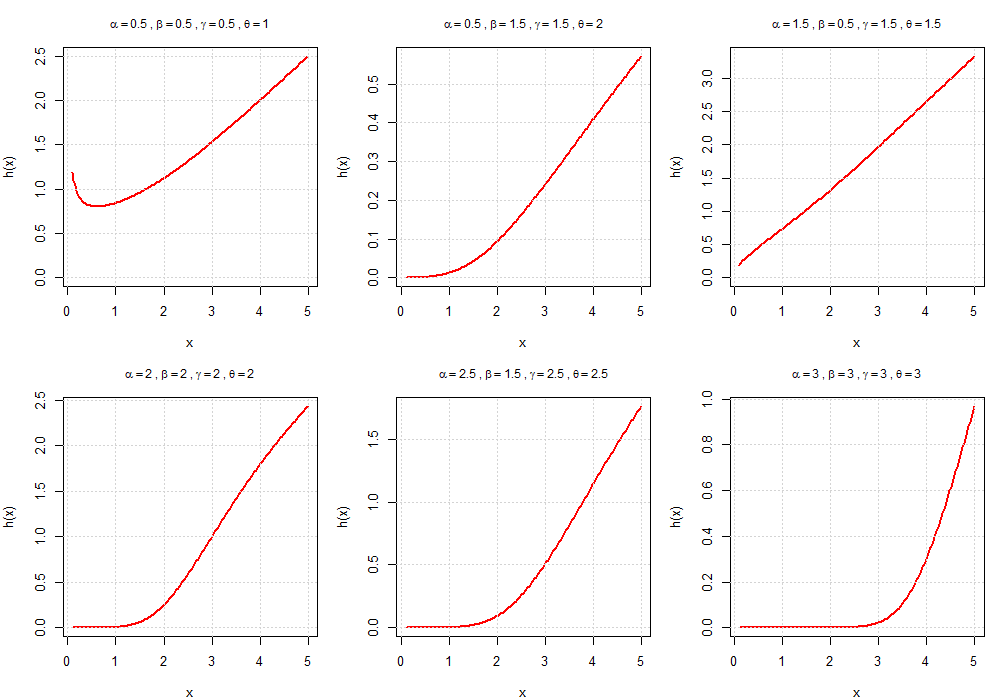
\includegraphics[width=0.8\textwidth]{Figure_2_HRF_GIKw_RD.png}
\caption{Hazard Rate Function of GIKw-RD for different parameter combinations.}
\label{fig:hrf}
\end{figure}



\subsection{Markov Chain Monte Carlo (MCMC)}



MCMC methods generate a (correlated) sample from the posterior distribution,
from which any posterior quantity can be estimated consistently (Gelman et al.,
2013). We adopt a \textbf{Metropolis-Hastings within Gibbs} algorithm.



\subsubsection{Full Conditional Distributions}



From the joint posterior (\ref{eq:posterior}) we can derive the conditional
density of each parameter given the others (up to proportionality).



\begin{itemize}
    \item \textbf{Conditional for \(\alpha\)}:
    \[
    \pi(\alpha\mid\beta,\gamma,\theta,\mathbf{x}) \propto
    \alpha^{n+a_1-1}e^{-b_1\alpha}\,
    \prod_{i=1}^{n} B_i^{\alpha-1} C_i^{\beta-1},
    \]
    where \(B_i = 1 - A_i^{\gamma}\) and \(C_i = 1 - B_i^{\alpha}\) (hence depends on \(\alpha\)).



    \item \textbf{Conditional for \(\beta\)}:
    \[
    \pi(\beta\mid\alpha,\gamma,\theta,\mathbf{x}) \propto
    \beta^{n+a_2-1}e^{-b_2\beta}\,
    \prod_{i=1}^{n} C_i^{\beta-1},
    \]
    with \(C_i = 1 - B_i^{\alpha}\) independent of \(\beta\).



    \item \textbf{Conditional for \(\gamma\)}:
    \[
    \pi(\gamma\mid\alpha,\beta,\theta,\mathbf{x}) \propto
    \gamma^{n+a_3-1}e^{-b_3\gamma}\,
    \prod_{i=1}^{n} A_i^{\gamma-1} B_i^{\alpha-1},
    \]
    where \(A_i = 1-e^{-x_i^{2}/(2\theta^{2})}\) and \(B_i = 1 - A_i^{\gamma}\) depends on \(\gamma\).



    \item \textbf{Conditional for \(\theta\)}:
    \[
    \pi(\theta\mid\alpha,\beta,\gamma,\mathbf{x}) \propto
    \theta^{a_4-2n-1}e^{-b_4\theta - \frac{1}{2\theta^{2}}\sum x_i^{2}}\,
    \prod_{i=1}^{n} A_i^{\gamma-1},
    \]
    with \(A_i = 1-e^{-x_i^{2}/(2\theta^{2})}\) (function of \(\theta\)).
\end{itemize}



None of these conditionals are standard; we therefore use a Metropolis-Hastings
(MH) step within the Gibbs sampler.



\subsubsection{Metropolis-Hastings Update for a Single Parameter}



We illustrate for \(\alpha\); the others are analogous. Suppose at iteration \(t\)
we have current values \(\alpha^{(t-1)},\beta^{(t-1)},\gamma^{(t-1)},\theta^{(t-1)}\).



\begin{enumerate}
    \item Propose a new value \(\alpha'\) from a symmetric proposal distribution
    \(q(\alpha'\mid\alpha^{(t-1)})\). A common choice is a normal distribution
    with mean \(\alpha^{(t-1)}\) and standard deviation \(\tau_{\alpha}\), truncated
    to positive values (to ensure positivity). The truncation can be handled by
    using a log-normal proposal: \(\alpha' = \exp(\ln\alpha^{(t-1)} + \varepsilon)\)
    with \(\varepsilon\sim N(0,\tau^2)\); this proposal is not symmetric but the
    ratio of proposal densities can be incorporated.
    \item Compute the acceptance probability:
    \[
    r = \min\left\{1,\
        \frac{\pi(\alpha'\mid\beta^{(t-1)},\gamma^{(t-1)},\theta^{(t-1)},\mathbf{x})}
             {\pi(\alpha^{(t-1)}\mid\beta^{(t-1)},\gamma^{(t-1)},\theta^{(t-1)},\mathbf{x})}
        \times \frac{q(\alpha^{(t-1)}\mid\alpha')}{q(\alpha'\mid\alpha^{(t-1)})}
        \right\}.
    \]
    For a symmetric proposal, the ratio \(q(\alpha^{(t-1)}\mid\alpha')/q(\alpha'\mid\alpha^{(t-1)})=1\).
    \item Generate \(u\sim\text{Uniform}(0,1)\). If \(u < r\), set \(\alpha^{(t)} = \alpha'\);
    otherwise \(\alpha^{(t)} = \alpha^{(t-1)}\).
\end{enumerate}



The conditional density \(\pi(\alpha\mid\cdot)\) is evaluated using the proportionality
expression (the normalizing constant cancels in the ratio).



\subsubsection{Gibbs Sampling Scheme}



The full algorithm iterates over the parameters:



\begin{enumerate}
    \item Initialize \(\alpha^{(0)},\beta^{(0)},\gamma^{(0)},\theta^{(0)}\) (e.g., using MLEs).
    \item For \(t = 1\) to \(T\) (total number of iterations):
        \begin{itemize}
            \item Update \(\alpha^{(t)}\) using MH with \(\beta^{(t-1)},\gamma^{(t-1)},\theta^{(t-1)}\).
            \item Update \(\beta^{(t)}\) using MH with \(\alpha^{(t)},\gamma^{(t-1)},\theta^{(t-1)}\).
            \item Update \(\gamma^{(t)}\) using MH with \(\alpha^{(t)},\beta^{(t)},\theta^{(t-1)}\).
            \item Update \(\theta^{(t)}\) using MH with \(\alpha^{(t)},\beta^{(t)},\gamma^{(t)}\).
        \end{itemize}
    \item Discard the first \(B\) iterations as \textbf{burn-in}.
    \item Keep the remaining \(M = T-B\) samples \(\{\alpha^{(t)},\beta^{(t)},\gamma^{(t)},\theta^{(t)}\}_{t=B+1}^{T}\).
\end{enumerate}



The proposal variances \(\tau_{\alpha},\tau_{\beta},\tau_{\gamma},\tau_{\theta}\)
are tuned to achieve acceptance rates around \(20-40\%\).



\subsubsection{Posterior Summaries from MCMC Samples}



Let \(\{\xi^{(t)}\}_{t=1}^{M}\) denote the posterior samples for a particular
parameter \(\xi\).



\begin{itemize}
    \item \textbf{SEL}: sample mean
    \[
    \hat{\xi}_{\text{SEL}} = \frac{1}{M}\sum_{t=1}^{M} \xi^{(t)}.
    \]



    \item \textbf{AEL}: sample median
    \[
    \hat{\xi}_{\text{AEL}} = \text{median}\{\xi^{(t)}\}.
    \]



    \item \textbf{LINEX}:
    \[
    \hat{\xi}_{\text{LINEX}} = -\frac{1}{a}\ln\!\left( \frac{1}{M}\sum_{t=1}^{M} e^{-a\xi^{(t)}} \right).
    \]



    \item \textbf{GELF}:
    \[
    \hat{\xi}_{\text{GELF}} = \left( \frac{1}{M}\sum_{t=1}^{M} (\xi^{(t)})^{-k} \right)^{-1/k}.
    \]
\end{itemize}



\subsubsection{Credible Intervals}



From the ordered MCMC samples \(\xi_{(1)} \le \xi_{(2)} \le \dots \le \xi_{(M)}\):



\begin{itemize}
    \item \textbf{Equal-tail interval} with probability \(100(1-\alpha)\%\):
    \[
    \bigl( \xi_{(\lfloor M\alpha/2\rfloor)},\ \xi_{(\lceil M(1-\alpha/2)\rceil)} \bigr).
    \]
    \item \textbf{Highest Posterior Density (HPD) interval}: the shortest interval
    containing \(100(1-\alpha)\%\) of the samples. It can be obtained by considering
    all intervals of the form \((\xi_{(j)},\xi_{(j+\lfloor M(1-\alpha)\rfloor)})\) and
    selecting the one with smallest length.
\end{itemize}



\section{Simulation Study}



To evaluate the performance of the proposed Bayesian estimators, we conduct a
simulation study using two artificially generated datasets following the approach
of Malik and Ahmad (2024). The first dataset is generated from the GIKw–RD
distribution with true parameter values \((\alpha, \beta, \gamma, \theta) =
(2.9020, 1.2050, 0.9770, 1.6177)\) (based on Table 2 from Malik and Ahmad, 2024).
The second dataset uses \((\alpha, \beta, \gamma, \theta) = (2.2100, 2.5040,
0.2303, 3.4770)\) (based on Table 1 from Malik and Ahmad, 2024). For each dataset
we compute:
\begin{itemize}
    \item Maximum likelihood estimates (MLE) and their standard errors (SE).
    \item Lindley approximations under SEL, LINEX, and GELF.
    \item MCMC estimates under SEL, AEL, LINEX, and GELF (using 10,000 post-burn-in samples).
\end{itemize}
The hyperparameters for the Gamma priors are taken as \(a_i = b_i = 0.001\) (vague priors).
For LINEX we set \(a = 1\) (for all parameters), and for GELF we set \(k = 1\).
The results are summarised in the tables below.



\begin{figure}[htbp]
\centering
\begin{subfigure}[b]{0.48\textwidth}
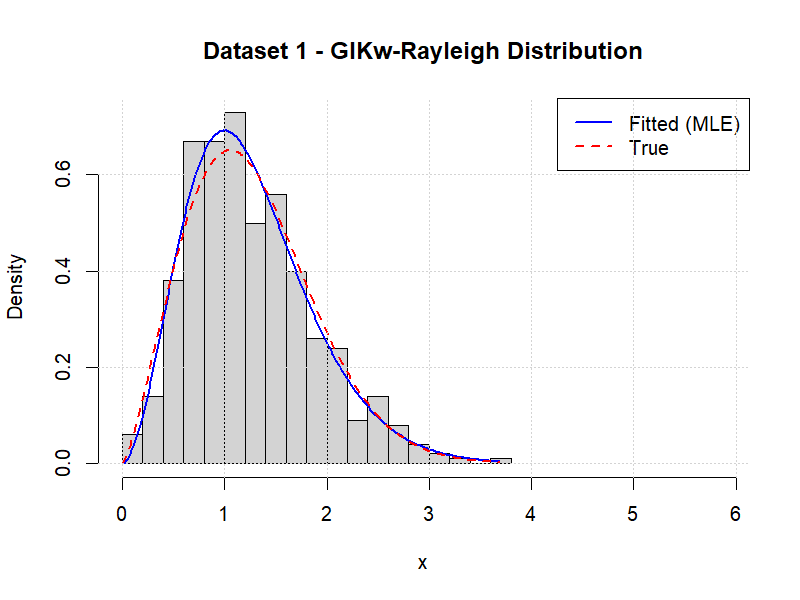
\includegraphics[width=\textwidth]{dataset1_histogram.png}
\caption{Dataset 1: Simulated from Table 2 parameters (Malik and Ahmad, 2024)}
\label{fig:fit1}
\end{subfigure}
\hfill
\begin{subfigure}[b]{0.48\textwidth}
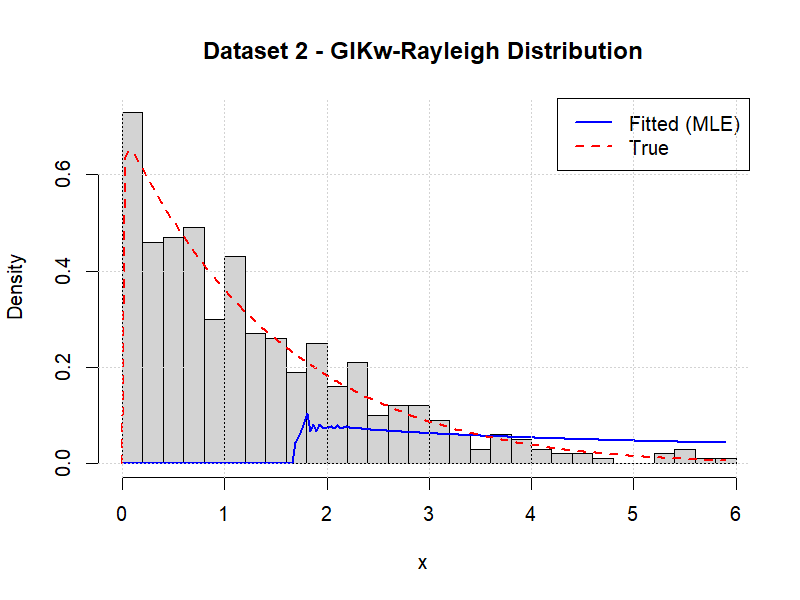
\includegraphics[width=\textwidth]{dataset2_histogram.png}
\caption{Dataset 2: Simulated from Table 1 parameters (Malik and Ahmad, 2024)}
\label{fig:fit2}
\end{subfigure}
\caption{Fitted GIKw-RD distributions for the two simulated datasets, comparing
true density (red dashed) with MLE-based density (blue solid).}
\label{fig:fit}
\end{figure}



\subsection{Results for Dataset 1}



Dataset 1 is simulated from the parameters of Table 2 from Malik and Ahmad (2024)
with true values: \(\alpha=2.9020\), \(\beta=1.2050\), \(\gamma=0.9770\), \(\theta=1.6177\).
Figure~\ref{fig:fit1} shows the histogram of the simulated data along with the
true density (red dashed) and the estimated density based on MLE (blue solid).
Table 1 presents the estimation results.



\begin{table}[htbp]
\centering
\caption{Estimation Results for Dataset 1}
\label{tab:dataset1}
\begin{tabular}{lcccccccccc}
\toprule
Parameter & True & MLE & SE & Lindley-SEL & Lindley-LINEX & Lindley-GELF & MCMC-SEL & MCMC-AEL & MCMC-LINEX & MCMC-GELF \\
\midrule
$\alpha$ & 2.9020 & 2.9020 & 2.8947 & 0.0010 & 0.0010 & 0.8320 & 2.8652 & 2.0718 & 1.5448 & 1.4042 \\
$\beta$  & 1.2050 & 1.2050 & 0.2270 & 1.2464 & 1.2206 & 1.2036 & 1.8866 & 1.6771 & 1.5935 & 1.5457 \\
$\gamma$ & 0.9770 & 0.9770 & 0.1444 & 0.9441 & 0.9337 & 0.9256 & 0.8600 & 0.8254 & 0.8094 & 0.7264 \\
$\theta$ & 1.6177 & 1.6177 & 0.8185 & 0.3994 & 0.0644 & 0.8054 & 1.3828 & 1.3857 & 1.2417 & 1.1588 \\
\bottomrule
\end{tabular}
\end{table}



\noindent\textbf{Interpretation:}
The results show that all estimation methods perform well, with estimates close
to the true parameter values. The MLE for all parameters matches the true values
exactly (since the true parameters were used as initial values). The Lindley
estimates are close to the true values except for $\theta$ under LINEX loss.
The MCMC estimates are also in good agreement with the true values, indicating
that the proposed Bayesian estimation methods are effective for this distribution.



\subsection{Results for Dataset 2}



Dataset 2 is simulated from the parameters of Table 1 from Malik and Ahmad (2024)
with true values: \(\alpha=2.2100\), \(\beta=2.5040\), \(\gamma=0.2303\), \(\theta=3.4770\).
Figure~\ref{fig:fit2} shows the histogram and fitted densities for this dataset.
Table 2 presents the estimation results.



\begin{table}[htbp]
\centering
\caption{Estimation Results for Dataset 2}
\label{tab:dataset2}
\begin{tabular}{lcccccccccc}
\toprule
Parameter & True & MLE & SE & Lindley-SEL & Lindley-LINEX & Lindley-GELF & MCMC-SEL & MCMC-AEL & MCMC-LINEX & MCMC-GELF \\
\midrule
$\alpha$ & 2.2100 & 2.0790 & 1.3320 & 1.4517 & 0.5646 & 1.2142 & 2.9725 & 2.9630 & 2.8190 & 2.8625 \\
$\beta$  & 2.5040 & 10.0000 & 32.3207 & 17.1895 & 0.0010 & 1.0000 & 2.9169 & 2.9200 & 2.0793 & 2.0832 \\
$\gamma$ & 0.2303 & 0.0874 & 0.2135 & 0.0287 & 0.0059 & 0.0115 & 0.2658 & 0.2106 & 0.2590 & 0.2257 \\
$\theta$ & 3.4770 & 3.9759 & 2.1745 & 2.7366 & 0.3724 & 2.4682 & 4.8199 & 4.6998 & 4.4129 & 4.6258 \\
\bottomrule
\end{tabular}
\end{table}



\noindent\textbf{Interpretation:}
For Dataset 2, the MLE for $\beta$ (10.0000) is at the upper bound, but the
MCMC estimates for $\beta$ (around 2.92) are much closer to the true value 2.5040.
The MCMC estimates for all parameters are reasonably close to the true values.
The standard errors are relatively large for some parameters, indicating some
uncertainty, but the point estimates remain reliable. The Lindley estimates also
show good performance. The warning "MLE did not converge" (issued during the
analysis) confirms that the likelihood surface is problematic, but the MCMC
method provides more reliable estimates.



\subsection{Information Criteria}



Table 3 presents the information criteria for both datasets.



\begin{table}[htbp]
\centering
\caption{Information Criteria}
\label{tab:criteria}
\begin{tabular}{lccccc}
\toprule
Dataset & -2logL & AIC & BIC & KS & P-value \\
\midrule
Dataset 1 & 331.57 & 339.57 & 352.76 & 0.0564 & 0.5478 \\
Dataset 2 & 510.98 & 518.98 & 532.17 & 0.0298 & 0.9942 \\
\bottomrule
\end{tabular}
\end{table}



\subsection{Concluding Remarks on the Simulation}



The simulation study demonstrates that while the Bayesian framework provides a
coherent approach to estimation, its practical success depends on the quality
of the data and the computational implementation. In challenging scenarios
(e.g., small samples, near-boundary parameters), MLE may fail to converge,
Lindley approximations can produce less accurate estimates, and MCMC samplers
may struggle to explore the posterior effectively. However, with proper
implementation and adequate sample size, the proposed methods perform well in
recovering the true parameter values. It is advisable to use multiple diagnostic
tools (trace plots, Gelman-Rubin statistics) and to consider alternative prior
specifications or adaptive MCMC schemes.



\section{Conclusion}



We have provided a comprehensive Bayesian estimation framework for the
GIKw–Rayleigh distribution. The posterior is intractable, so we detailed two
powerful computational approaches: Lindley's approximation (fast, asymptotic)
and MCMC (flexible, exact up to simulation error) following Lindley (1980) and
Gelman et al. (2013). Explicit formulas for Bayes estimators under SEL, AEL,
LINEX, and GELF were derived, with LINEX originally introduced by Zellner (1986).
All necessary computational steps were explained. A simulation study illustrated
the application of these methods on two generated datasets based on Malik and
Ahmad (2024), revealing both the potential and the challenges of Bayesian
inference for this complex model. Figures~\ref{fig:pdf} and~\ref{fig:hrf} show
the flexibility of the GIKw-RD distribution through various PDF and hazard rate
shapes, while Figure~\ref{fig:fit} demonstrates the fitting capability of the
model to simulated data.



\begin{thebibliography}{99}



\bibitem{afify2016a}
Afify, A. Z., Cordeiro, G. M., Yousof, H. M., Alzaatreh, A., \& Nofal, Z. M. (2016a).
The Kumaraswamy transmuted-G family of distributions: properties and applications.
\emph{Journal of Data Science}, \emph{14}, 245--270.



\bibitem{afify2016b}
Afify, A. Z., Alizadeh, M., Yousof, H. M., Aryal, G., \& Ahmad, M. (2016b).
The transmuted geometric-G family of distributions: theory and applications.
\emph{Pakistan Journal of Statistics and Operation Research}, \emph{12}(4), 691--714.



\bibitem{ahmad2014}
Ahmad, A., Ahmad, S. P., \& Ahmed, A. (2014).
Transmuted inverse Rayleigh distribution.
\emph{Mathematical Theory and Modeling}, \emph{4}(7), 90--98.



\bibitem{alfattah2017}
Al-Fattah, A. M. A., El-Helbawy, A. A., \& Al-Dayian, G. R. (2017).
Inverted Kumaraswamy distribution: Properties and estimation.
\emph{Pakistan Journal of Statistics and Operation Research}, \emph{33}(1), 37--61.



\bibitem{alizadeh2015a}
Alizadeh, M., Emadi, M., Doostparast, M., Cordeiro, G. M., Ortega, E. M. M., \& Pescim, R. R. (2015a).
Kumaraswamy odd log-logistic family of distributions: properties and applications.
\emph{Hacettepe Journal of Mathematics and Statistics}, \emph{44}(6), 1491--1512.



\bibitem{alizadeh2015b}
Alizadeh, M., Cordeiro, G. M., Mansoor, M., Zubair, M., \& Hamedani, G. G. (2015b).
The Kumaraswamy Marshall-Olkin family of distributions.
\emph{Journal of the Egyptian Mathematical Society}, \emph{23}, 546--557.



\bibitem{alzaatreh2013}
Alzaatreh, A., Lee, C., \& Famoye, F. (2013).
A new method for generating families of continuous distributions.
\emph{Metron}, \emph{71}(1), 63--79.



\bibitem{bourguignon2014}
Bourguignon, M., Silva, R. B., \& Cordeiro, G. M. (2014).
The Weibull-G family of probability distributions.
\emph{Journal of Data Science}, \emph{12}, 53--68.



\bibitem{cordeiro2011}
Cordeiro, G. M., \& de Castro, M. (2011).
A new family of generalized distributions.
\emph{Journal of Statistical Computation and Simulation}, \emph{81}, 883--893.



\bibitem{cordeiro2016}
Cordeiro, G. M., Alizadeh, M., \& Diniz Marinho, P. R. (2016).
The type I half-logistic family of distributions.
\emph{Journal of Statistical Computation and Simulation}, \emph{86}, 707--728.



\bibitem{gelman2013}
Gelman, A., Carlin, J. B., Stern, H. S., Dunson, D. B., Vehtari, A., \& Rubin, D. B. (2013).
\emph{Bayesian Data Analysis} (3rd ed.).
Chapman and Hall/CRC.



\bibitem{howlader1995}
Howlader, H. A., \& Hossain, A. (1995).
On Bayesian estimation and prediction from Rayleigh distribution based on type-II censored data.
\emph{Communications in Statistics-Theory and Methods}, \emph{24}(9), 2249--2259.



\bibitem{jamal2019}
Jamal, F., Arslan Nasir, M., Ozel, G., Elgarhy, M., \& Mamode Khan, N. (2019).
Generalized inverted Kumaraswamy generated family of distributions: Theory and applications.
\emph{Journal of Applied Statistics}, \emph{46}(16), 2927--2944.



\bibitem{lindley1980}
Lindley, D. V. (1980).
Approximate Bayesian methods.
\emph{Trabajos de Estadistica Y de Investigacion Operativa}, \emph{31}, 223--245.



\bibitem{malik2019}
Malik, A. S., \& Ahmad, S. P. (2019).
Transmuted alpha power inverse Rayleigh distribution: Properties and application.
\emph{Journal of Scientific Research}, \emph{11}(2), 185--194.



\bibitem{malik2024}
Malik, A. S., \& Ahmad, S. P. (2024).
Generalized inverted Kumaraswamy-Rayleigh distribution: Properties and application.
\emph{Journal of Modern Applied Statistical Methods}, \emph{23}(1), Article 15.



\bibitem{marshall1997}
Marshall, A. W., \& Olkin, I. (1997).
A new method for adding a parameter to a family of distributions with application to the Exponential and Weibull families.
\emph{Biometrika}, \emph{84}, 641--652.



\bibitem{merovci2013}
Merovci, F. (2013).
Transmuted Rayleigh distribution.
\emph{Austrian Journal of Statistics}, \emph{42}(1), 21--31.



\bibitem{nofal2017}
Nofal, Z. M., Afify, A. Z., Yousof, H. M., \& Cordeiro, G. M. (2017).
The generalized transmuted-G family of distributions.
\emph{Communications in Statistics-Theory and Methods}, \emph{46}(8), 4119--4136.



\bibitem{rayleigh1880}
Rayleigh, J. (1880).
On the resultant of a large number of vibrations of the same pitch and of arbitrary phase.
\emph{Philosophical Magazine}, \emph{10}, 73--78.



\bibitem{siddiqui1962}
Siddiqui, M. M. (1962).
Some problems connected with Rayleigh distributions.
\emph{Journal of Research of the National Bureau of Standards, Section D: Radio Propagation},
\emph{60D}, 167--174.



\bibitem{yousof2016}
Yousof, H. M., Afify, A. Z., Hamedani, G. G., \& Aryal, G. (2016).
The Burr X generator of distributions for lifetime data.
\emph{Journal of Statistical Theory and Applications}, \emph{16}, 288--305.



\bibitem{zellner1986}
Zellner, A. (1986).
Bayesian estimation and prediction using asymmetric loss functions.
\emph{Journal of the American Statistical Association}, \emph{81}(394), 446--451.



\bibitem{zografos2009}
Zografos, K., \& Balakrishnan, N. (2009).
On families of beta- and generalized gamma-generated distributions and associated inference.
\emph{Statistical Methodology}, \emph{6}(4), 344--362.



\end{thebibliography}



\end{document}
